\documentclass[11pt,french,a4paper]{article}
\usepackage[utf8]{inputenc}
\usepackage[french]{babel}
\usepackage[T1]{fontenc}
\usepackage{fancyhdr}
\usepackage{fancybox}
\usepackage{lastpage}
\usepackage{graphicx}
\usepackage[left=2cm,right=2cm,top=2cm,bottom=2.5cm]{geometry}
\geometry{a4paper}
\setlength{\parindent}{0pt}
\usepackage{listings}
\usepackage{color}
\usepackage[table]{xcolor}
\usepackage{array}
\usepackage{listings}
\usepackage{hyperref}
\usepackage{caption}
\usepackage{lastpage}
\pagestyle{fancy}

\fancyhead[L]{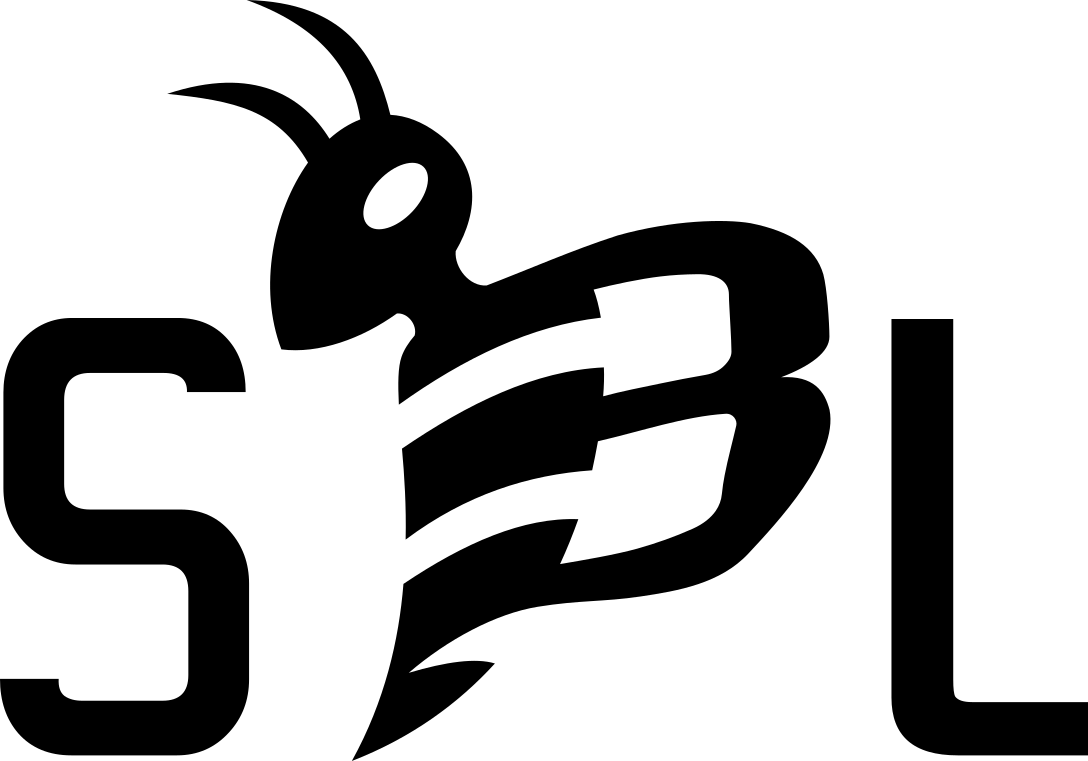
\includegraphics[width=1cm]{../../../logo/SBLlogo.png}}
\fancyhead[C]{Rapport d'activiter semaines du 11 et 18 avril 2022 }
\fancyhead[R]{}
\fancyfoot[L]{\small Tom TUELEAU\normalsize}
\fancyfoot[C]{}
\fancyfoot[R]{\thepage/\pageref{LastPage}}


\lstset{
  basicstyle=\fontfamily{lmvtt}\selectfont\small,
  columns=fullflexible,
}

\title{
 \centering
         
\includegraphics[width=4cm]{../../../logo/IUTlogo.png}  \hspace{7cm}
         
\includegraphics[width=4cm]{../../../logo/UMlogo.png}  \hspace{7cm}
    
	\LARGE{Rapport d'activiter du 11 et 18 avril 2022}
	\author{TUELEAU Tom}
}
\author{
	\date{}
}
\begin{document}
\maketitle
	 
\includegraphics[width=4cm]{../../../logo/LIRMMlogo.png}  \hspace{7cm}
         \includegraphics[width=4cm]{../../../logo/IBMMlogo.jpg}  \hspace{7cm}
\newpage
\tableofcontents
\newpage
\section{Introduction}
Ce document a pour objectif de faire un état d'avancement du stage. Celui-ci résumera donc le travail effectué lors des semaines du 11 et 18 avril 2022.
\\Je vais vous présenter dans un premier temps les recherche que j'ai pu effectuer sur le Piezo-Electrique les AOP ou encore la fréquence qu'émettent les abeilles. 
\\Dans une deuxième partie,je parlerait de la découverte du logiciel spice ainsi que les simulation que j'ai pu effectué lors de ces 2 semaines.
\\Une troisiéme partie reviendras sur les résultats obtenue pour le capteur de vibration. 
\\Enfin, une dernière partie introduira les outil que j'ai mis en place pour m'organiser tout aux long du projet. 

\newpage
\section{Recherche}
Comme dis en introduction, j'ai été amener à me documenter afin d'accomplire plusieur objectifs. Le premier objectif était d'étudier solution à ma disposition afin d'amplifier mon signal. Mes rechercher ce sont donc porter sur les amplificateur operationel. Mon second objectif était de faire des recherche sur le fréquence émise par les abeilles afin de commander des capteur de vibrations avec une plage de fréquence adéquate. 
\subsection{AOP}
Ma principal source d'information pour cette partie à été Mr Druon m'ayant fournis plusieur documentation fiable sur les montage à amplificateur opérationel. 
Mes recherche on donc principalement concister à tester des montages et à verifier par le calcul si les valeur récupéré était les bonnes.
Je suis donc passer directement à de l'experimentation en testent comme vue lors du précédent rapport différents montages basique.
Nous verrons plus en détail lors de la partie "Capteur de vibration" la mise en pratique de ces montages.

\subsection{Fréquence et piezo-electrique}
Afin de pouvoire mesurer avec plus de précision les vibration émise par les abeilles, j'ai pris conseil au pres de monsieur Rouset qui m'a fourni different article sur le sujet.
Apres une lecture de ces document, je suis arriver à une estimation de la plage de fréquence de communication des abeilles dans la ruche à [200Hz-1000Hz]. Je me base sur cette echange avec Mr ROUSSET pour déduire cette plage de valeurs : \\ 
\\
\\
\fbox{
	\begin{minipage}{17cm} 
Les vibrations dans les matériaux qui sont probablement détectées par plusieurs organes/structures dans le corps de l’abeille. Par exemple l’organe subgénual (subgenual organ) localisé dans la patte est sensible aux vibrations entre 200 et 1000Hz.
	\end{minipage}

}
\\ \\ \\Etant donner le temps restent avent la dead-line j'ai préferer me baser sur ce résultat pour la commande des piézo-électrique.

\newpage
\section{Simulation}
Afin de pouvoire simuler les montage qu'il me seras nécessaire d'effectuer, il m'a été conseiller d'étudier et de me former sur le logiciel spice.

\subsection{ngspice}
Étant sur une distribution linux j'ai installer le logiciel "ngspice". Cellui-ci est Open Source et est installable trés facilement sur n'import qu'elle distribution baser sur Unix. L'objectif principal pour moi est de pouvoire simuler mes montages afin d'étudier leur comportement. 

\subsection{Apprentisage du logiciel}
Lors de cette semaine d'apprentisage de spice j'ai pu apprendre les chose suivante :
\\
- Simuler un cicuit de base avec resistor, condensateur, bobine, générateur de tension, génerateur de courent\\
- Créer un signal continue, sinusoidale et impulsionel \\
- Afficher les résultat de ceci à l'aide de graphique \\
\\

\subsection{Etats actuel}
Malgres le temps investie sur cellui-ci je ne maitrise pas encore parfaitement le logiciel et suis encore entrein de le prendre en main. Je compte cependant tenter dans la semaine à venire, de simuler le montage que vous verrez dans la prochaine partie. 
\newpage
\section{Capteurs de vibration}
Le capteur piezo-electrique ne produisant pas une tension asser élever pour que je l’utilise tel qu’elle, j’ai donc du trouver un moyen de l’amplifier. Je vais donc vous présentez les montages que j’ai pu étudier et les résultats obtenus.

\subsection{Montage}
\subsubsection{Rappel}

Comme vue dans le rapport de la premier semaine, j’ai commencer par faire des montages basiques (Suiveur, Amplificateur non-inverseur) avec composer d’amplificateur operationel (AOP). Ceux-ci m’avais  posser des problemes due aux modeles d’AOP que j’utilise (LM741) qui nécesite une alimentation en paraléle.

\subsubsection{Amplificateur de mesure}

Lors de cette semaine je suis donc passer au montage amplificateur de mesure. Ce montage est très souvent utilisé afin d’amplifier le signal de sortie d’un capteur aillant une tension trop faible.
Il existe plusieurs montages amplificateur de mesures. Dans mon cas, j’ai commencer par un montage necesitant 3 AOP. Nous pouvons voire ce montage figure \ref{3AOP}

\begin{center}	
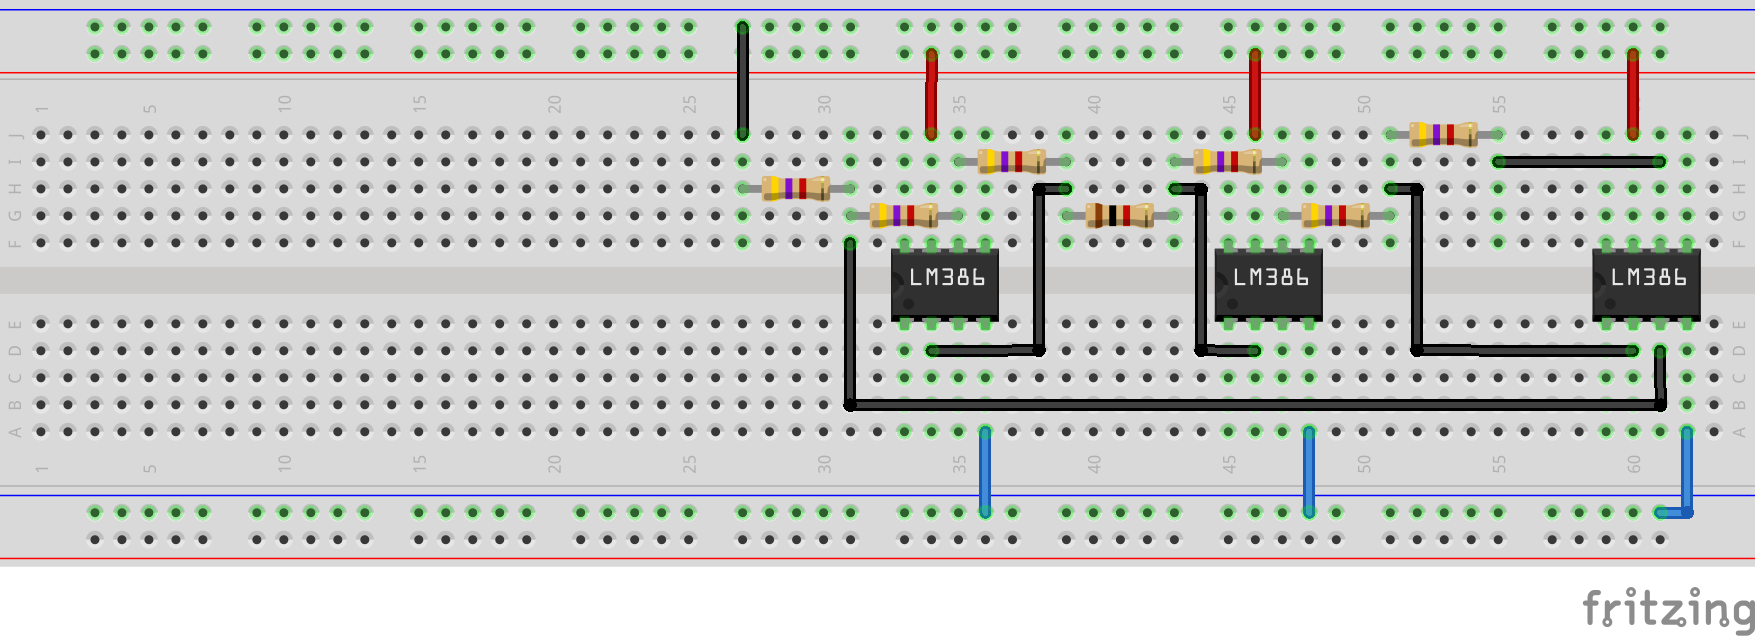
\includegraphics[scale=1]{../img/instrumentation3aop_bb.png}
\captionof{figure}{Montage 3 AOP sous Fritzing}
\label{3AOP}
\end{center}


Il existe cepdendent des montages plus simple notament un composer de deux amplificateur opératione que l'on peut voire figure \ref{2AOP}.
\\

\begin{center}	
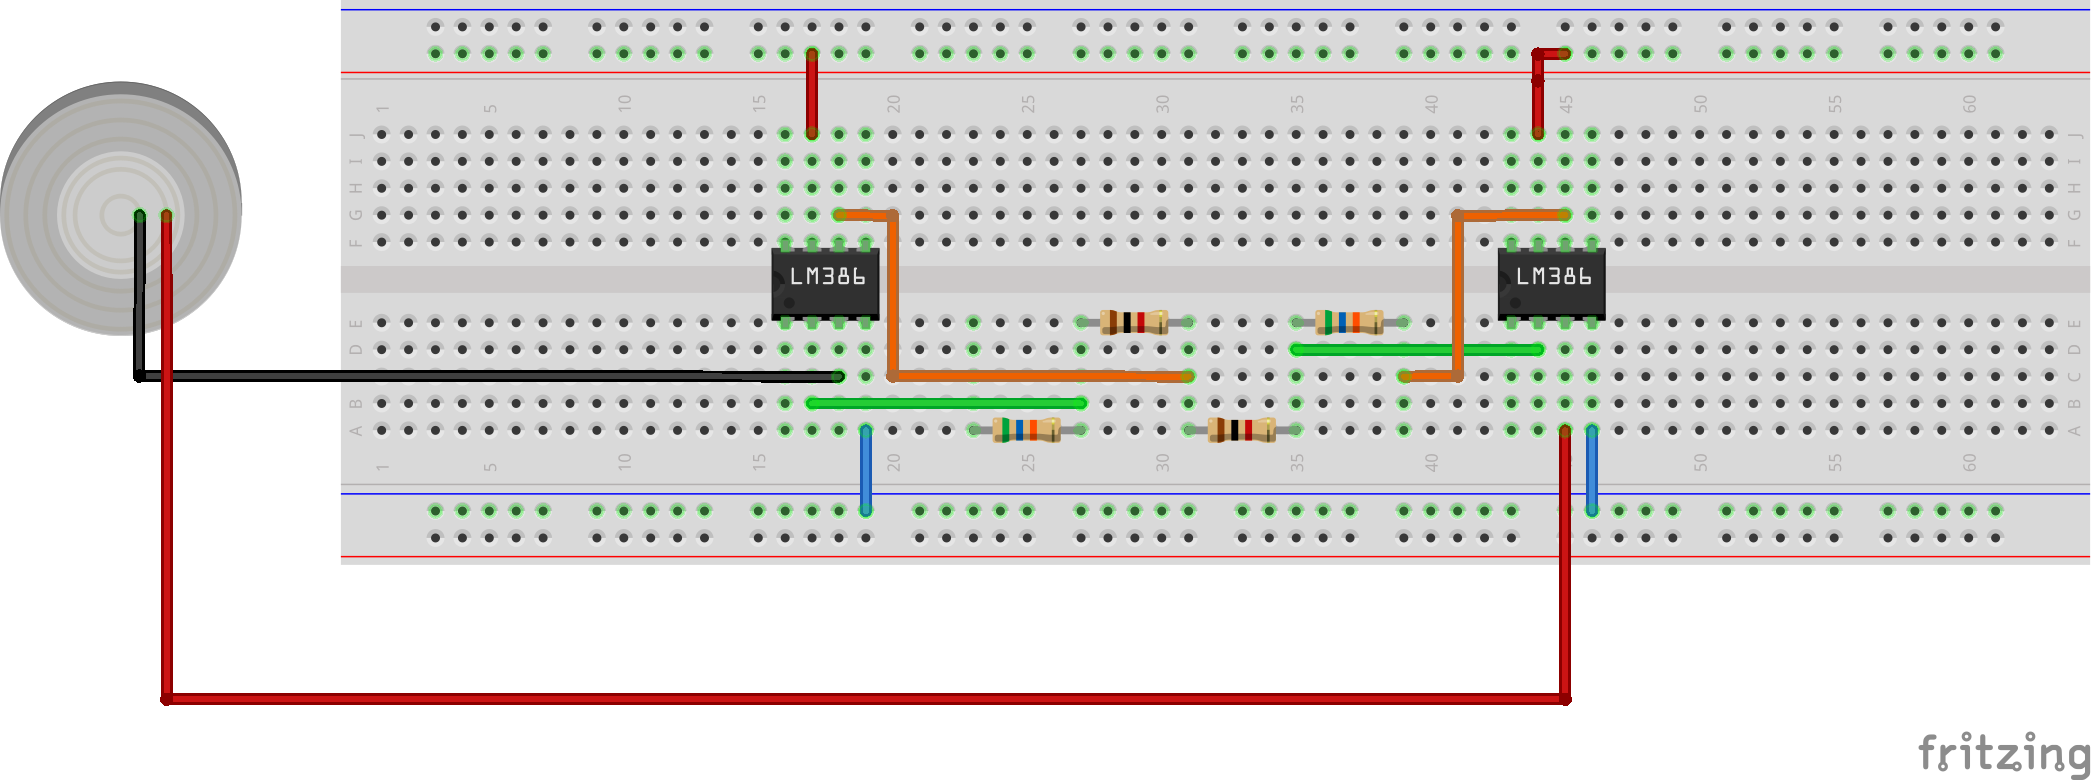
\includegraphics[scale=0.80]{../img/instrumentation2aop_bb.png}
\captionof{figure}{Montage 2 AOP sous Fritzing}
\label{2AOP}
\end{center}

Aprés avoire réussit à effectuer ce montage, j’ai pu remarquer que la sensibiliter avais diminuer. Ceci a eux pour effet de d’enpecher la visions d’impulsion créer lors de petit frotement. Aprés plusieurs tentative de modification pour pallier à ce changement, j’ai désidé de changer de montage.

\subsubsection{Montage actuel}
Le piezo-electrique utilisé jusqu’a maintenantétait fournis avec un module en plus. Cellui-ci ne changais rien aux signal pour cause, les composant sur lui n’etait pas totalement connecter. Cependant apres avoire effectuer des modification sur cellui-ci le signal ma parus beaucoup plus net.
J’ai par la suite effecuter le montage visible figure \ref{MTGFINAL}
\\
\begin{center}	
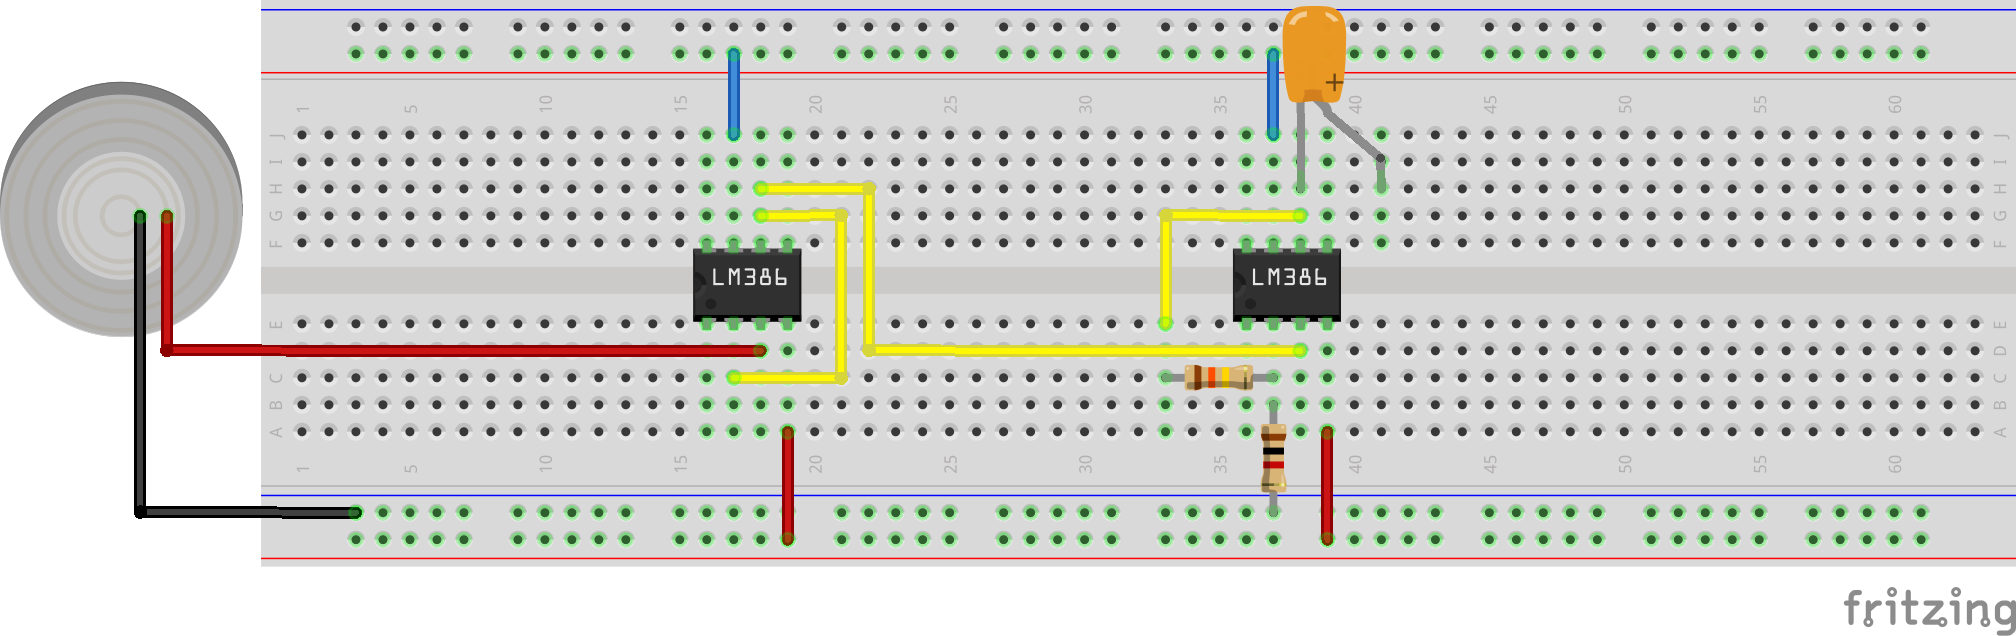
\includegraphics[scale=0.85]{../img/mtgfinal.png}
\captionof{figure}{Dernier montge }
\label{MTGFINAL}
\end{center}
Il est composer d’un amplificateur suiveur et d’un amplificateur non-inverseur avec un coeficient multiplicateur de 130. C'est à dire que la tension de sortie seras 130 fois la tension d'entrer. Enfin un condensateur ce trouvent en sortie de circuit nous permet d’éliminer la composante continue ajouter par les AOP à notre signal.


\subsubsection{Résultat}
Avec le montage vue précédemment nous obtenont plusieurs résultat probant.
Tout d'abords nous pouvont voir figure \ref{VWOMVM} le signal en sortie du montage quand aucun évenement ne ce produit.
Ensuite figure \ref{F} nous pouvons voire la réaction apres un léger frotement effectuer avec un cable visible figure \ref{M}. 

\begin{center}	
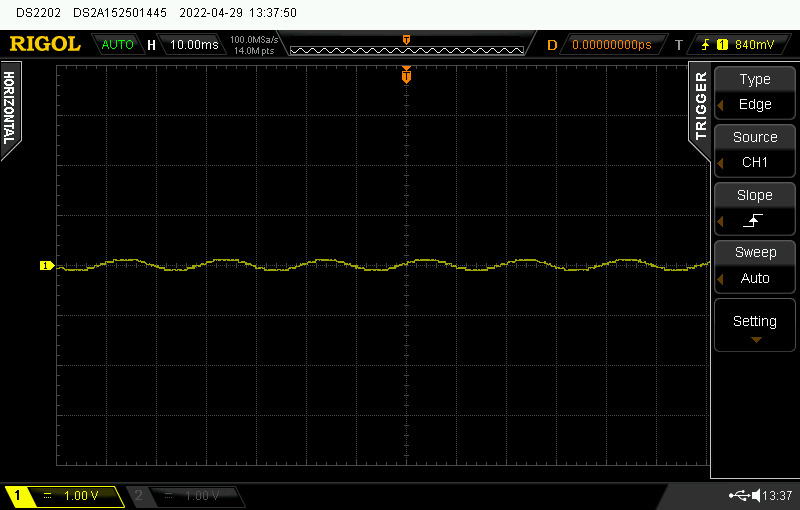
\includegraphics[scale=0.5]{../img/plat.jpg}
\captionof{figure}{Tension sans mouvement}
\label{VWOMVM}
\end{center}

\begin{center}	
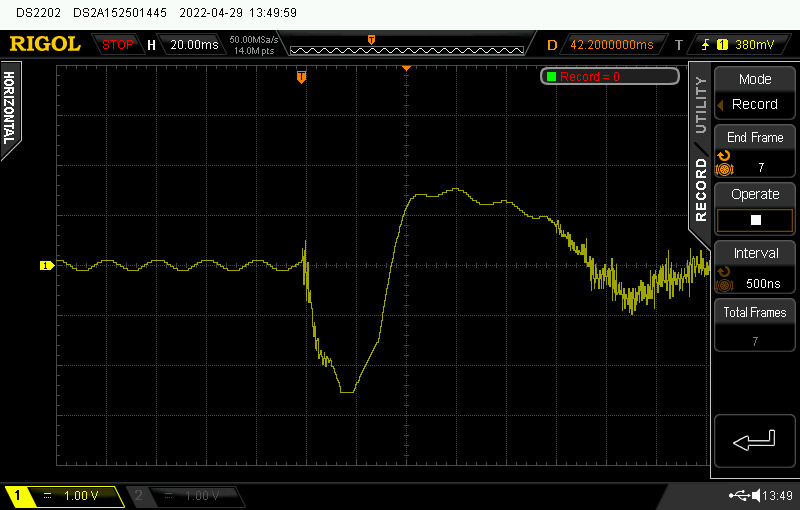
\includegraphics[scale=0.5]{../img/frotment.jpg}
\captionof{figure}{Tension lors d'un Frotement}
\label{F}
\end{center}

\begin{center}	
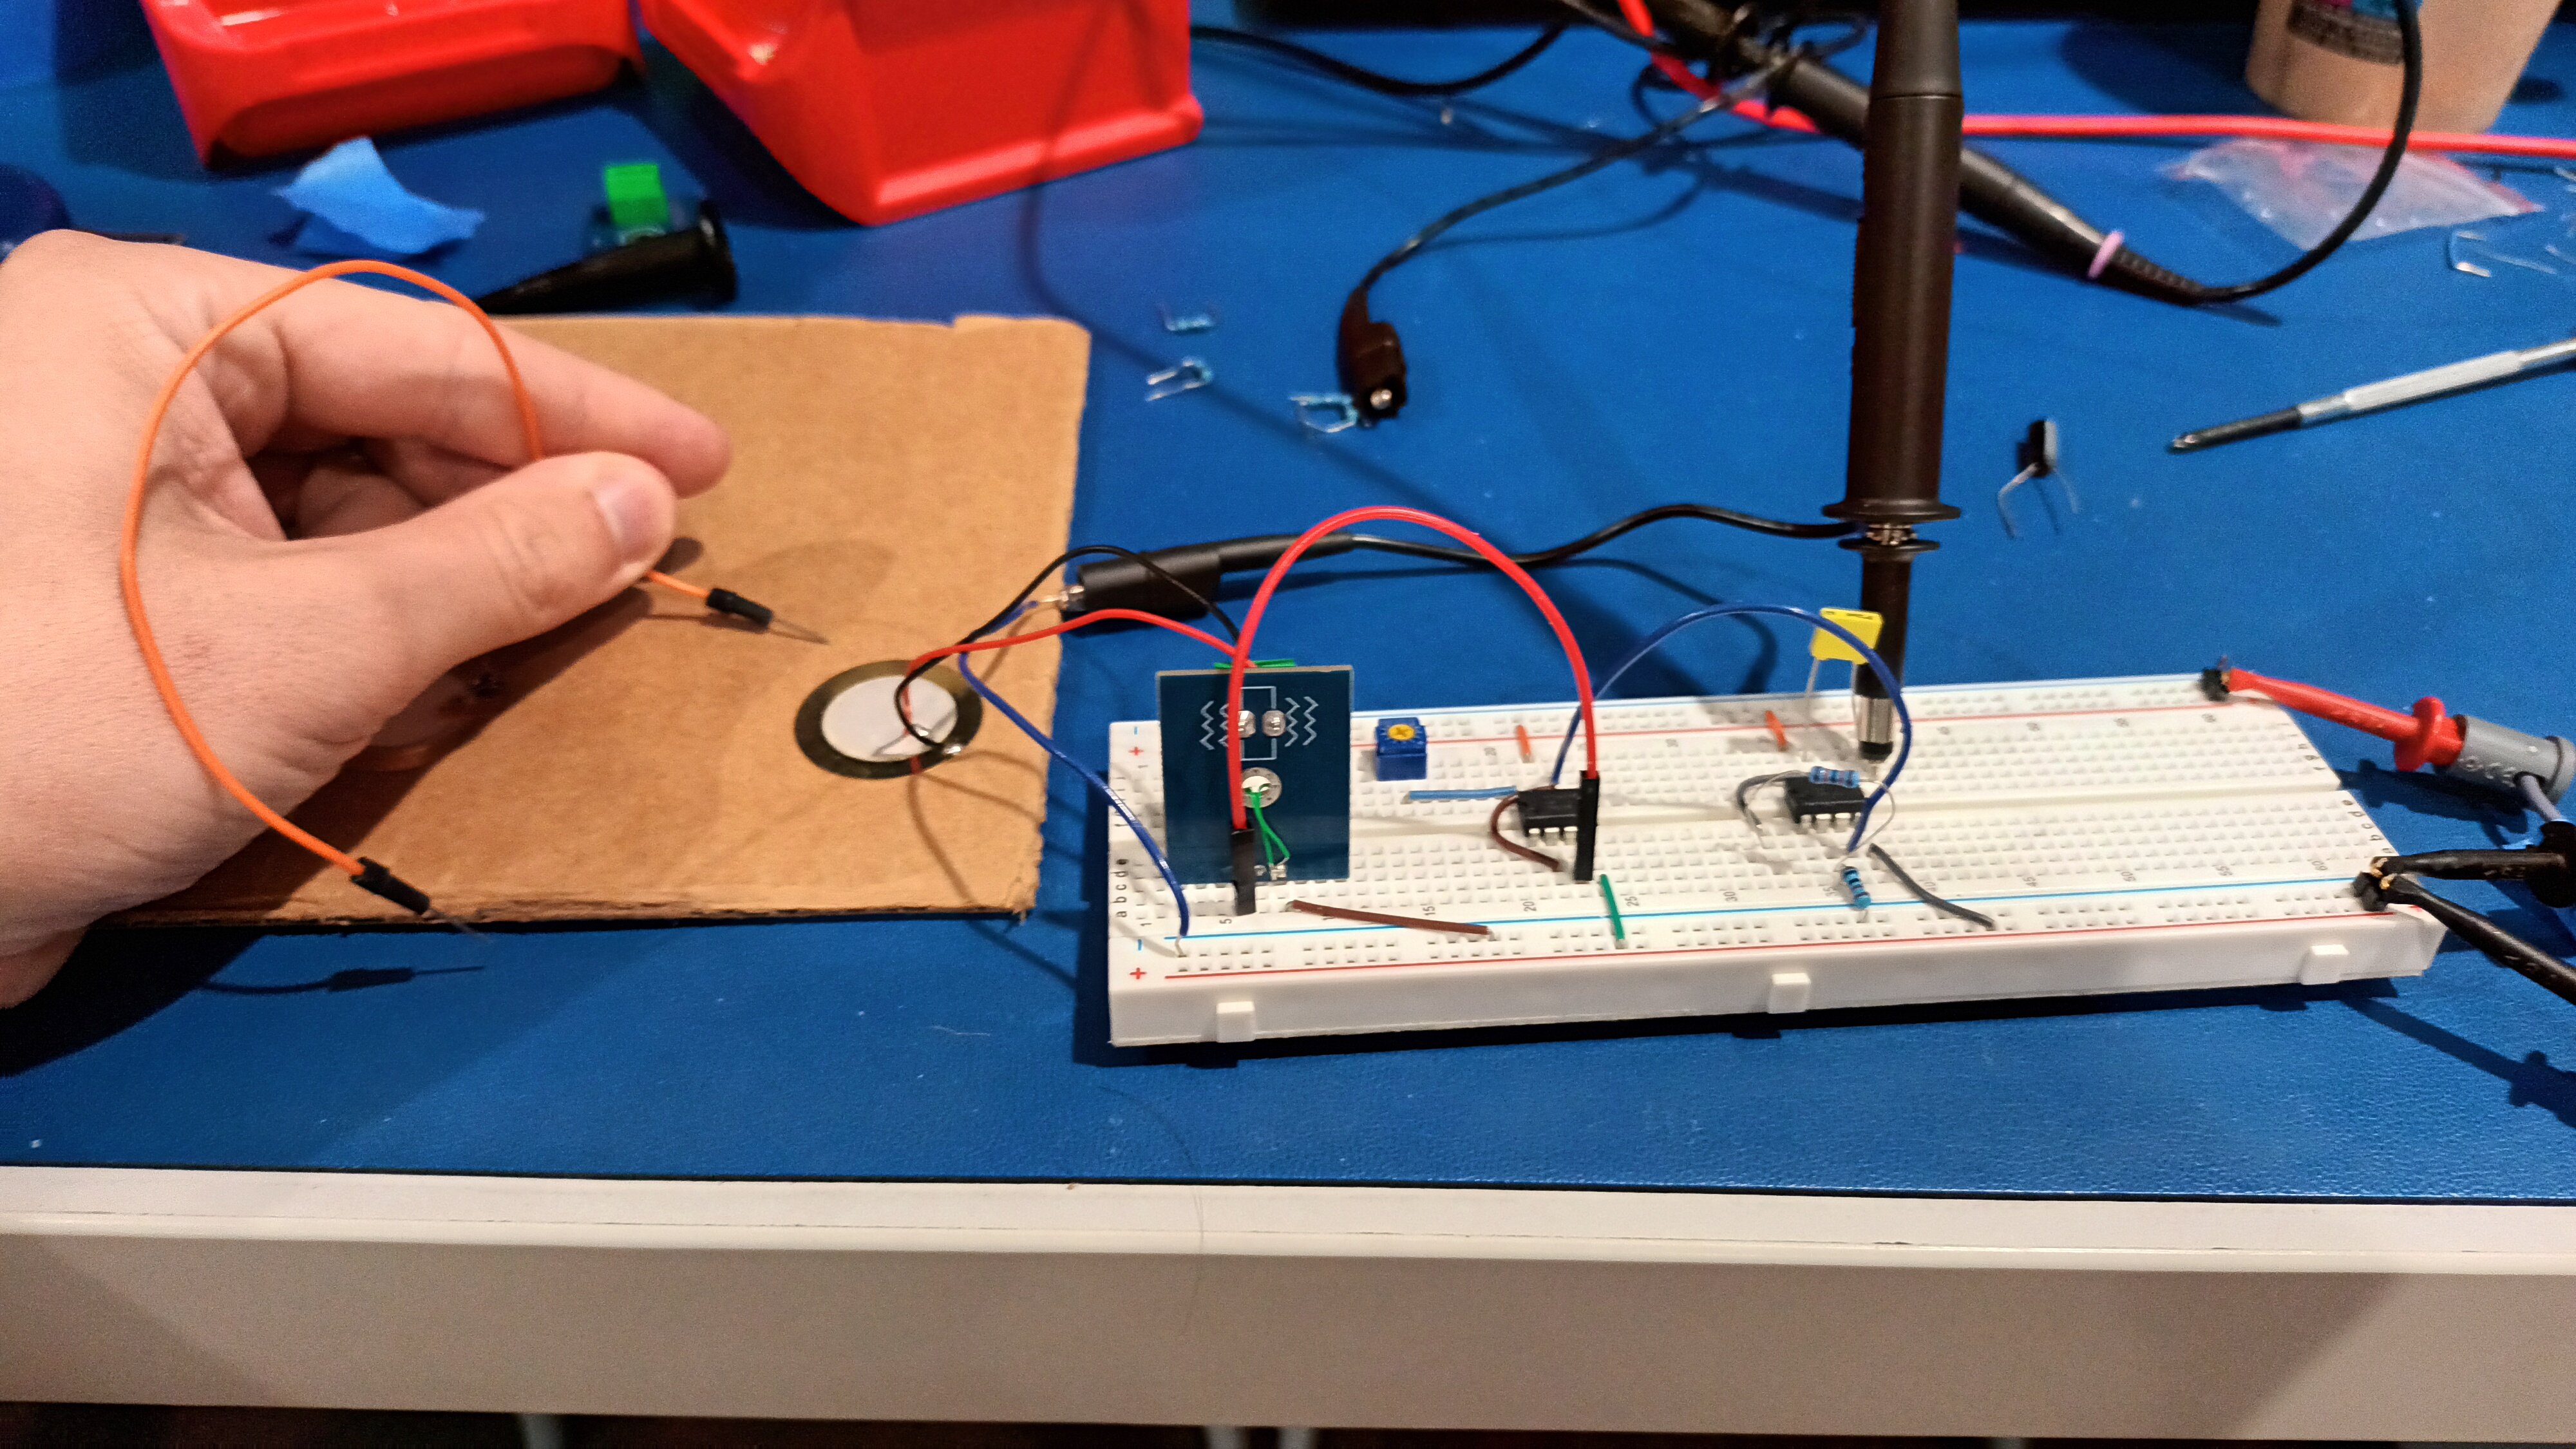
\includegraphics[scale=0.1]{../img/froty.jpg}
\captionof{figure}{Frotement}
\label{M}
\end{center}

\subsubsection{Conclusion}
Nous somme donc passer d’une tension de l’ordre dont l’interval était [50-90mV] à une intervalle de [0,6-1,5V]. Ces valleurs seront bien plus exploitable et permetrons le traitement via l’arduino.
Cependant le montage montrer ci-dessus ne seras pas le final. Il me faut encore produire un montage plus propre et a traiter la partie numérisation du signal.

\newpage
\section{Gestion}
Afin de pouvoire m'organiser et avoire un suivis de mon acctiviter tout aux long du stage, j'ai mis en place un gantt sous la forme d'une page Notion.

\subsection{Organisation de l'espace }
Chaque page que j'ai créer sur notion posséde une fonction précis. Je vais donc vous présent brievement chacune d'entre elles.
\subsubsection{Calendrier}

Comme sont nom l'indique la page calendrier répertorie chaque tache ayant été effectué sous la forme d'un calendrier. Celle-ci me permet de m'organiser sur le mois à venir et surout à garder un oeil sur mes dead-line. 
\begin{center}	
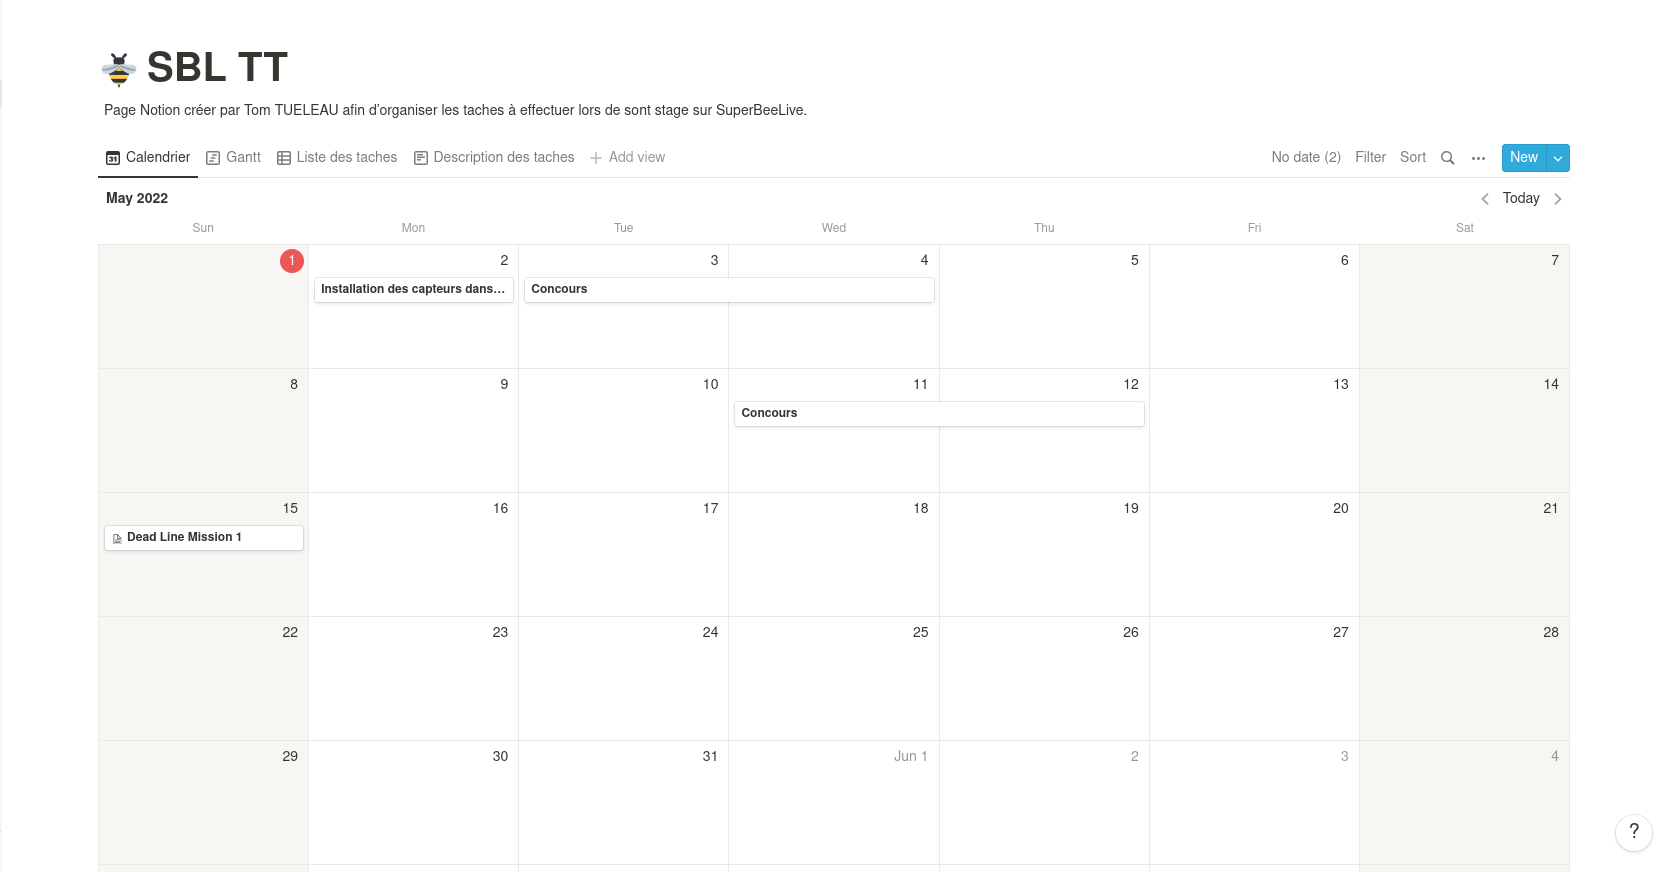
\includegraphics[scale=0.35]{../img/notioncalender.png}
\captionof{figure}{Calendrier}
\label{Calendrier}
\end{center}

\subsubsection{Liste des taches}
La page liste des taches regroupe toute les taches effectuer et a efféctuer. J'attribue à ces taches des étiquettes ce qui me permet des les classer.   
\begin{center}	
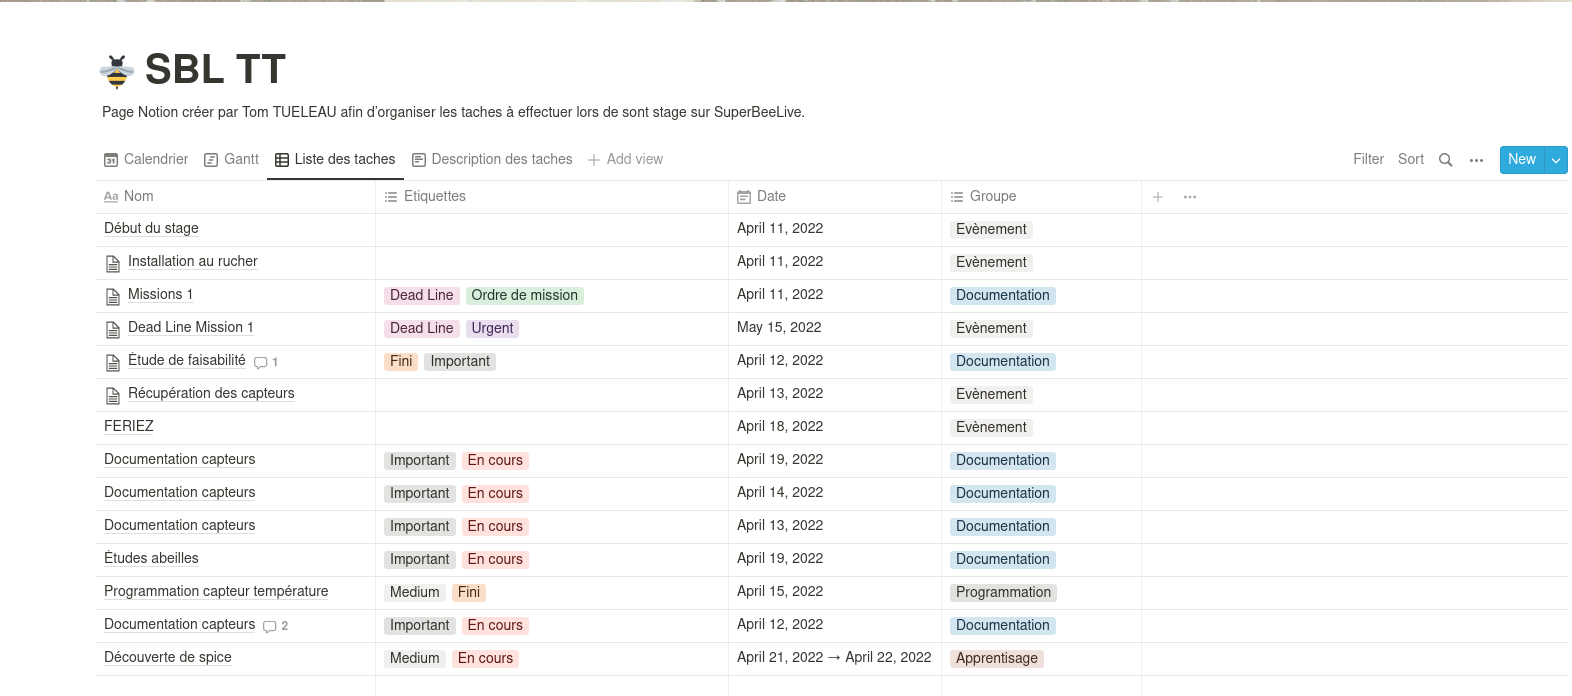
\includegraphics[scale=0.35]{../img/notionlistesdestaches.png}
\captionof{figure}{Liste des taches}
\label{Liste des taches}
\end{center}

\subsubsection{Description des taches}
Cette onglet contient une description plus détailler des taches. J'y stoque aussi les compte rendue de réunion, prise de note, image relative à mes partie du projet.
\begin{center}	
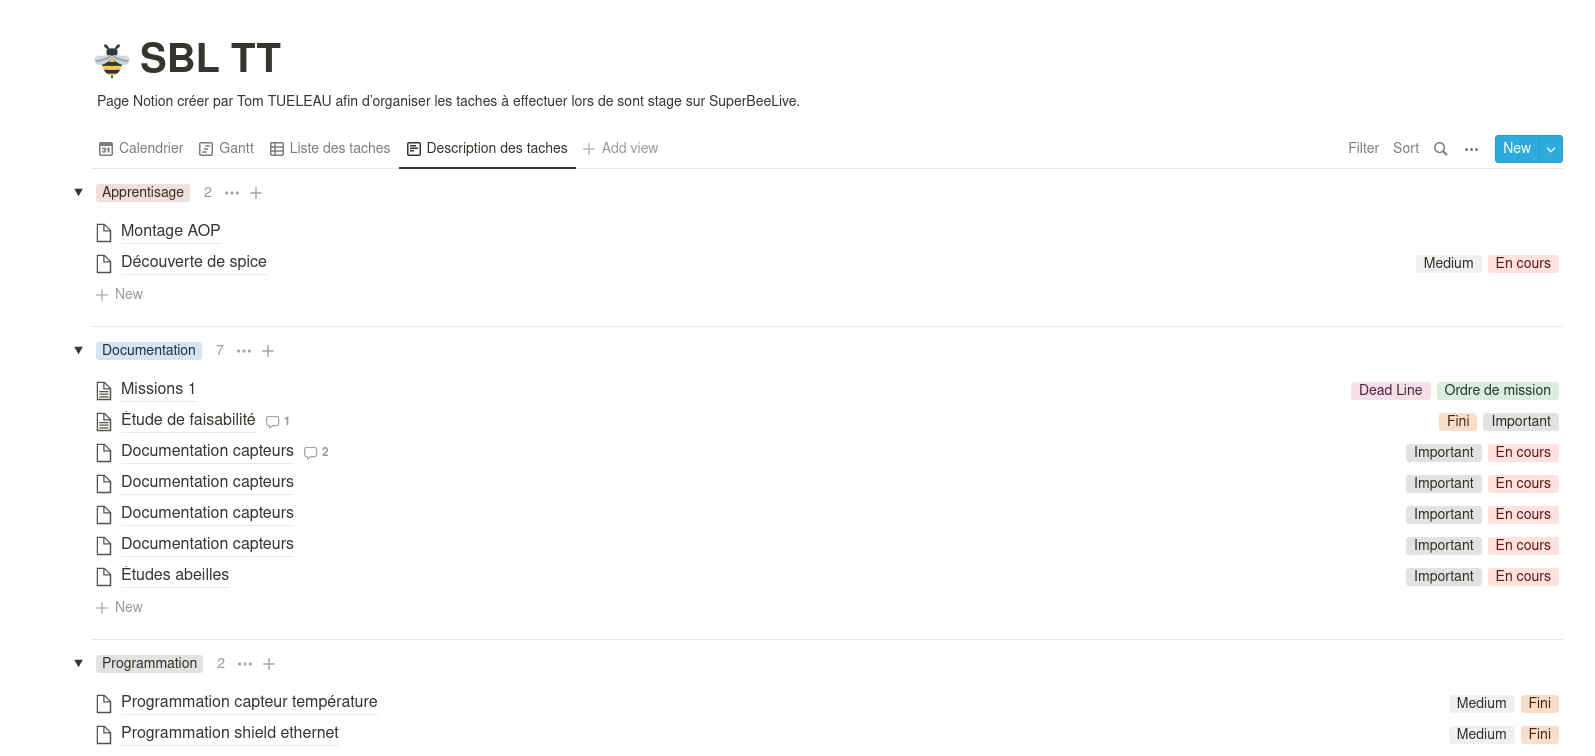
\includegraphics[scale=0.35]{../img/notiondescriptiondestaches.png}
\captionof{figure}{Description des taches}
\label{Description des taches}
\end{center}

\subsubsection{Gantt}
La dernier fiche accessible est la fiche "Gantt" qui me permet surout de m'organiser sur ma semaine. 
\begin{center}	
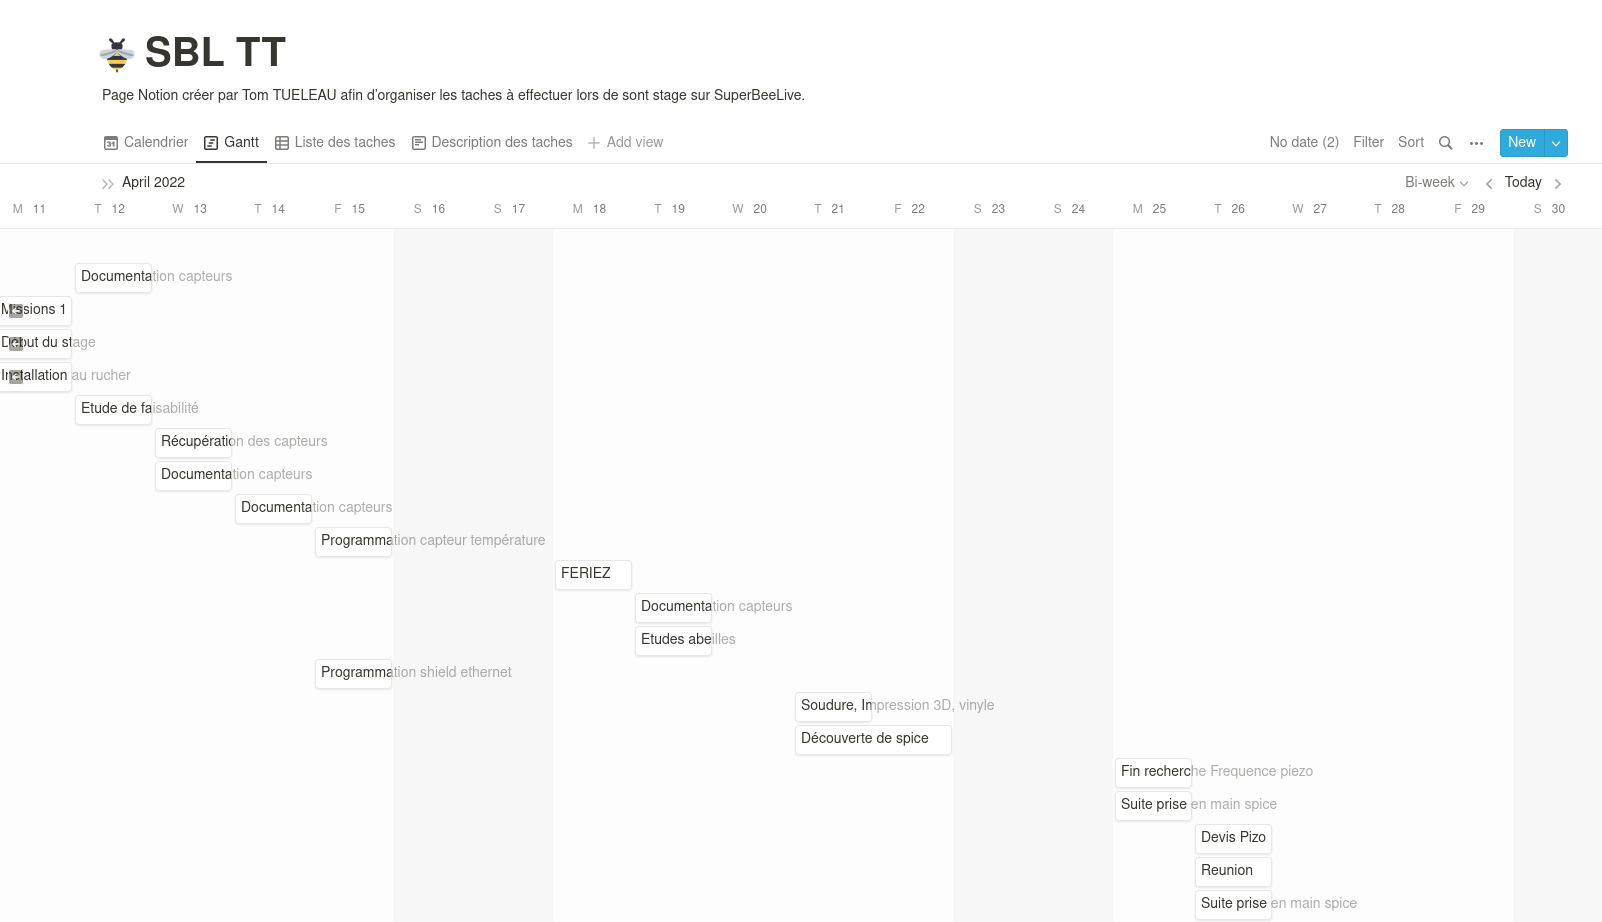
\includegraphics[scale=0.35]{../img/notiongantt.png}
\captionof{figure}{Gantt}
\label{Gantt}
\end{center}
\newpage 
\section{Conclusion}

Les taches qu'il me reste à effectuer pour les prochaine semaines sont les suivantes :
\\
\\- Mettre en place dans la ruche les capteurs déjà opérationel
\\- Rendre opérationel le capteur de vibration en finalisant sur une plaquette de prototypage le montages d'amplification.
\\- Organiser l'affichage des données avec la personne charger du site Web. 
\\- Reprendre l'annalyse du logiciel "Jaaba" de  Kristin Branson. 
\\- Regarder et mettre en fonctionnement le microphone fournis.
\newpage
\listoffigures
\end{document}
